\chapter{Lecture 7 - Rankine Cycle with Closed Feedwater Heaters}
\label{ch:ch7}
\section{Objectives}
The objectives of this lecture are:
\begin{itemize}
\item Describe Closed Feedwater Heaters (CFWH)
\item Discuss the ``Cascade Back'' and ``Pump Forward'' arrangements for dealing with CFWH drains.
\item Provide some design and modeling notes.
\end{itemize}

\section{Closed Feedwater Heaters}
\newthought{In a previous lecture} we learned about open feedwater heaters (OFWH).  OFWHs are used in the Rankine Cycle to pre-heat feedwater before entering the Steam Generator.  In workshop exercises you could see how use of OFWHs reduce overall exergy destruction (irreversibility) and improve cycle thermal efficiency.  

Closed feedwater heaters (CFWHs) perform the same role.  The differences is that in CFWHs the fluids do \underline{not} mix.  A simple schematic is given in Figure \ref{fig:CFWH_1}.
\begin{marginfigure}
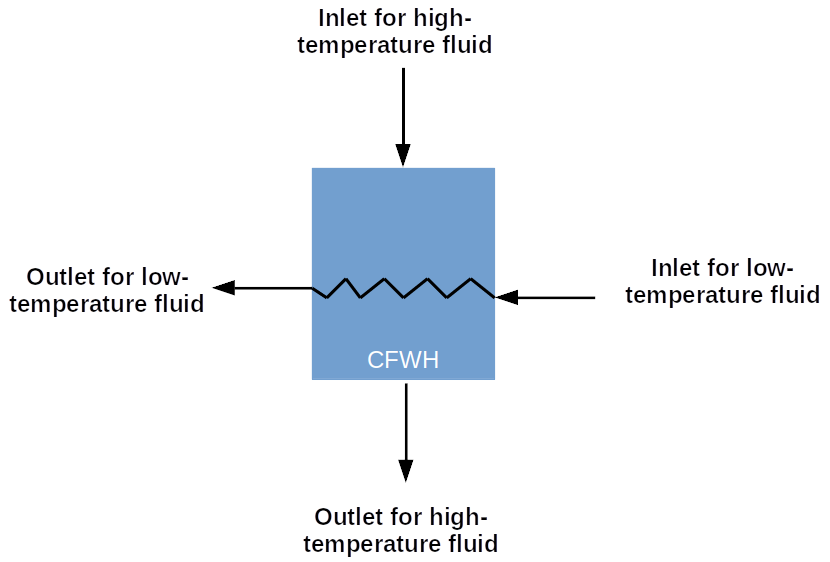
\includegraphics{CFWH_simple_schematic.png}
\caption{Simple CFWH schematic.}
\label{fig:CFWH_1}
\end{marginfigure}
\newthought{The high-temperature fluid} is normally steam, extracted from a selected turbine stage, and the low-temperature fluid being heated is normally feedwater.  The low-temperature water is, for all of our applications, a subcooled liquid.  The high-temperature fluid is, for most nuclear applications, a saturated mixture of relatively high quality ($x \ge 80$ percent) although in principle it could be superheated.  The outlet for high temperature fluid is normally a saturated or slightly subcooled liquid. For CFWHs the outlet of the low temperature fluid is usually still a subcooled liquid albeit at a higher temperature than it was at the inlet. 

Although it is beyond the scope of this class, it is worthwhile to consider the added complexity of modeling---and at some point in our career designing---a heat exchanger where one of the fluids undergoes phase changes.  A somewhat more realistic schematic representation of a CFWH is showing in Figure \ref{fig:CFWH_2}.  Here, in the case that the extraction steam is above saturation temperature, the steam is reduced to saturation temperature in the ``de-superheater'' region on the heat exchanger.  Heat transfer correlations used for single-phase convective heat transfer from the steam to the heat exchanger tubes would be used to model heat exchanger performance.  In the ``condenser'' region, the complicated phase change process occurs where steam is converted to saturated liquid.  In the ``condensate cooler'' region, once again single-phase heat transfer prevails as the liquid water gives up its energy to the incoming feed flow.

\begin{marginfigure}
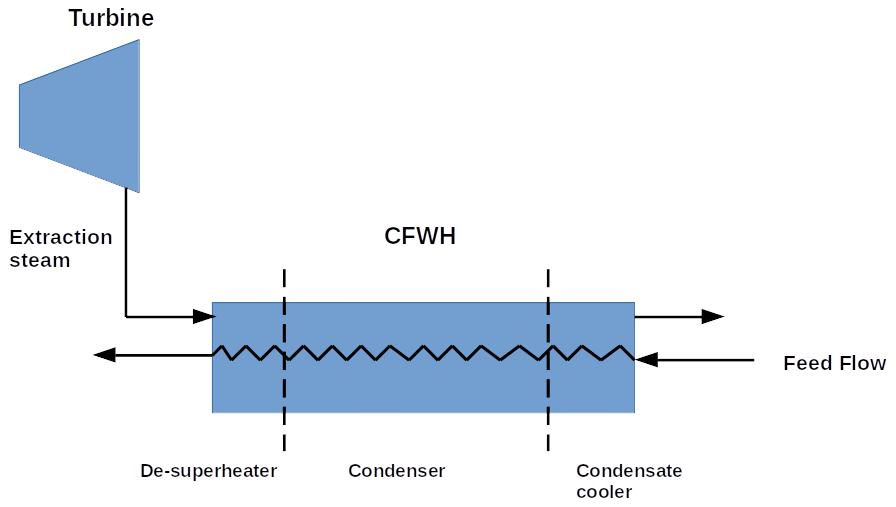
\includegraphics{CFWH_schematic.png}
\caption{Conceptual schematic of a CFWH.}
\label{fig:CFWH_2}
\end{marginfigure}


\newthought{Once the heating fluid} exits the CFWH, it has to go somewhere.  In OFWHs, the heating fluid was simply carried away with the (now preheated) feedwater.  In a CFWH, the high-temperature fluid exit needs to be directed somewhere else to be integrated into the feed-flow stream.  There are two conventional choices for doing this:
\begin{enumerate}
\item ``Drain Cascade Back''---type 1
\item ``Drain Pump Forward''---type 2
\end{enumerate}

The Rankine cycle schematic shown in Figure \ref{fig:RC_MS_RH_OFWH_CFWH_t1} illustrates a type 1 arrangement.
\begin{figure}
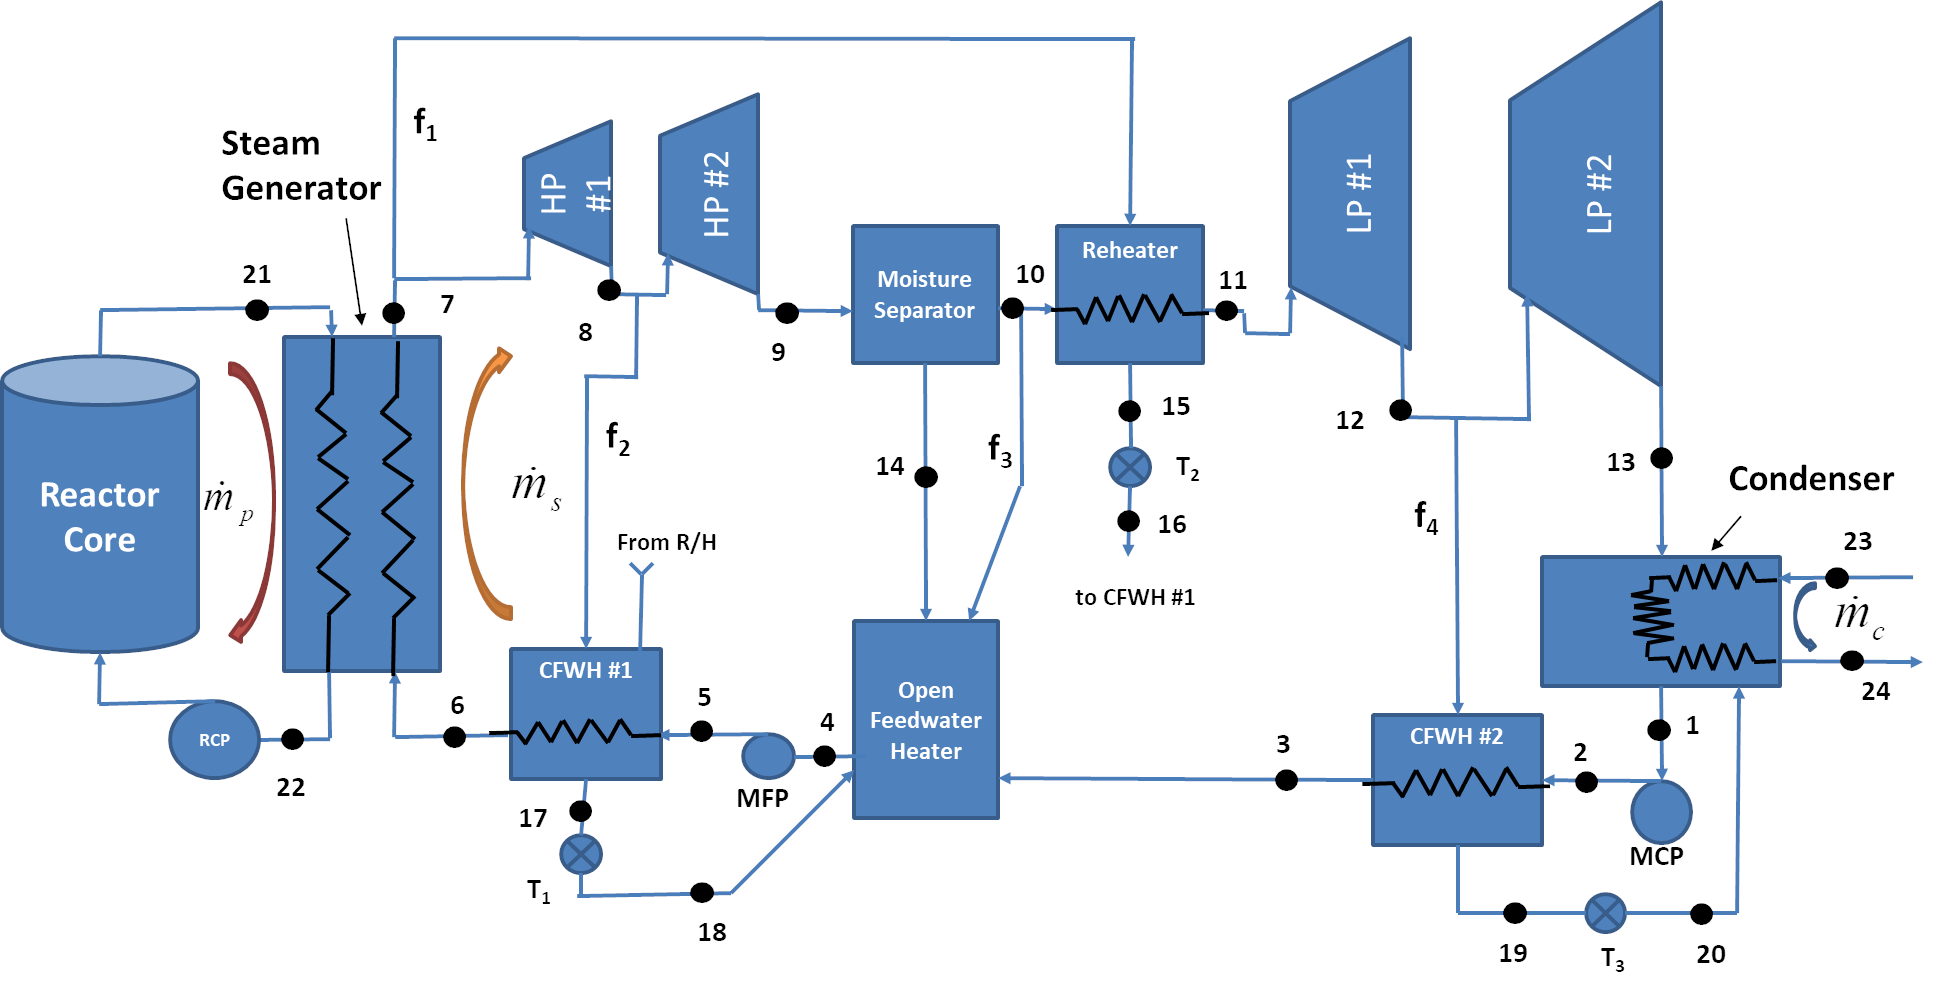
\includegraphics{Rankine_with_MS_RH_OFWH_CFWH_type1.png}
\caption{Complex Rankine cycle with type 1 ``Drain Cascade Back'' CFWH arrangement.}
\label{fig:RC_MS_RH_OFWH_CFWH_t1}
\end{figure}
CFWH \#1 has two high-temperature fluid inputs: one is extraction steam from the turbine labeled ``HP \#1''; the other comes from the re-heater exit.\marginnote[-0.5cm]{\textbf{Question: }Why is it probably better to direct the fluid at state point 16 to CFWH \#1 rather than to the OFWH, CFWH \#2, or the Condenser?}  The heating fluid in the CFWH all exits through a common drain.  This drain is directed to the OFWH.  Since all fluids entering the OFWH must be at the same pressure, this fluid is expanded through a trap (labeled $T_1$) entering the OFWH at state point 18.

\newthought{A cycle with multiple} CFWHs will normally cascade the heat exchanger drains in order to extract maximum reheating benefit from the extraction steam.  A simplified schematic of Rankine cycle employed with the Experimental Breeder Reactor II is presented in Figure \ref{fig:EBRII}.\cite{koch2008experimental}
\begin{figure}
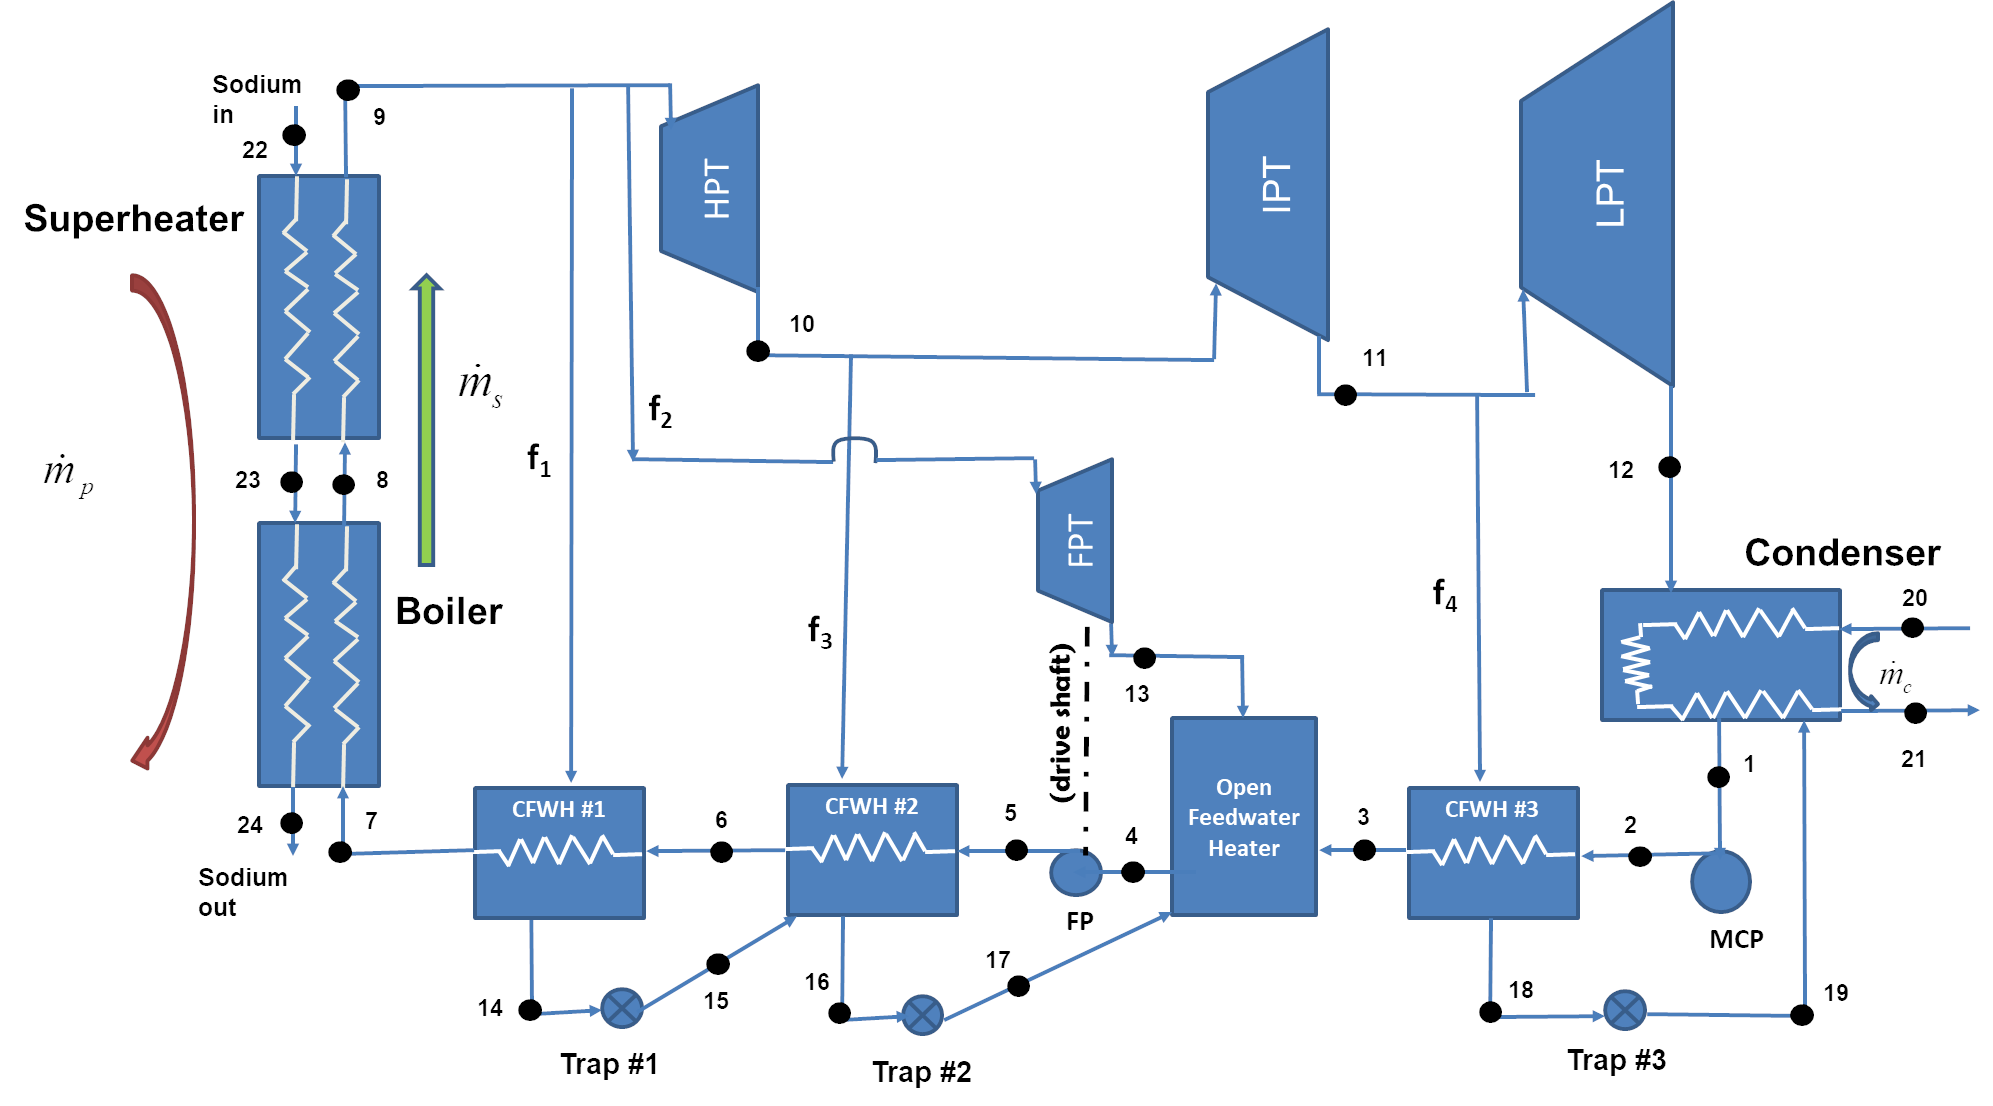
\includegraphics{EBR_II.png}
\caption[][1cm]{Simplified schematic of the Experimental Breeder Reactor II energy conversion cycle with cascaded CFWH drains.}
\label{fig:EBRII}
\end{figure}


\newthought{A type 2 arrangement} for a CFWH is illustrated in Figure \ref{fig:CFWH_type2}.  Notice the extra state point required at the exit of the CFWH after the point where the drain pump discharge is mixed in to the feedwater flow.  
\begin{marginfigure}
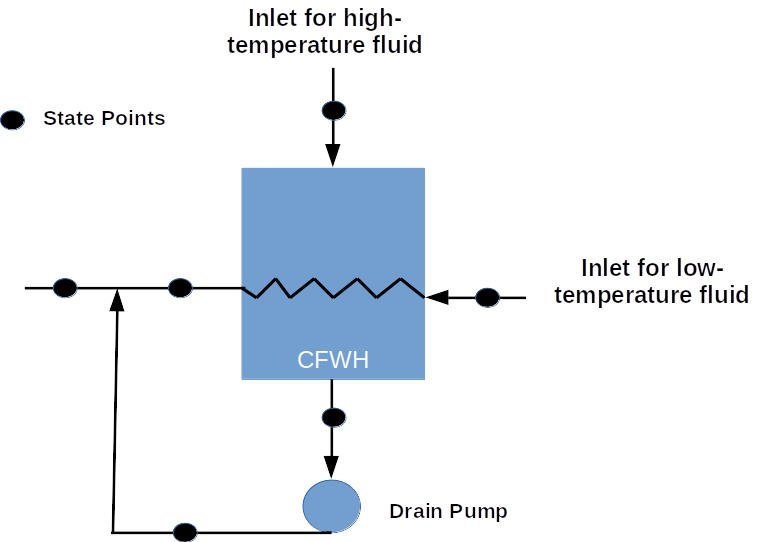
\includegraphics{Pump_Forward_CFWH_Drain.png}
\caption{Schematic of CFWH with type 2 drain pump arrangement.}
\label{fig:CFWH_type2}
\end{marginfigure}




\section{Design and Modeling Notes}
There are too many details on the variations of Rankine cycle designs in order to hope to cover them all in one course, much less one lecture.  Here I provide a set of bullet-points to try and summarize some general principles that one can get by examining modern and relevant Rankine cycles for nuclear energy conversion:

\begin{itemize}
\item Rankine cycles typically utilize a mixture of OFWHs and CFWHs (e.g. 5-6 CFWHs + 1 or 2 OFWHs).  
\item BWRs generally will not use OFWHs due to the need to contain gaseous radionuclides in the coolant.\sidenote{OFWHs usually include a dearator function where air and other non-condensable gasses are vented from the feedwater and ejected to the atmosphere. In a BWR some of those gasses may be radioactive.}  
\item High pressure / low temperature outlet from the CFWH is usually modeled as having the same (or nearly the same) temperature as the incoming heating steam.  
\item High temperature / low pressure outlet from CFWH is usually modeled as a saturated liquid (or slightly sub-cooled).
\item Extraction steam pressures are often chosen such that the steam temperature (in each extraction stream) is reduced in roughly equal increments.
\item ``Drain Pumped Forward'' CFWHs result in slightly higher thermal efficiency but:
\begin{enumerate}
\item Requires another pump (that might break); and
\item Combinations of drain-forward and drain cascade back possible (of course).
\end{enumerate}
\item How much is it worth to increase thermal efficiency a little bit by adding all of this complexity:
\begin{itemize}
\item For a navy nuclear powered warship?
\item for a commercial nuclear power plant operator?
\end{itemize}
\end{itemize} 

